To improve the performance of the STREAM Triad kernel for both CPUs and GPUs, we can compute on a range of data elements that can be processed in parallel, by converting the loop to a parallel\_for kernel.\par

A STREAM Triad kernel may be trivially executed on a CPU by submitting it into a queue for a parallel execution. The body of this STREAM Triad DPC++ parallel kernel looks exactly like the body of the STREAM Triad loop that executes in serial C++ on the CPU, as shown in Figure 16-6.\par

\hspace*{\fill} \par %插入空行
Figure 16-6. DPC++ STREAM Triad parallel\_for kernel code
\begin{lstlisting}[caption={}]
constexpr int num_runs = 10;
constexpr size_t scalar = 3;

double triad(
		const std::vector<double>& vecA,
		const std::vector<double>& vecB,
		std::vector<double>& vecC ) {
			
	assert(vecA.size() == vecB.size() == vecC.size());
	const size_t array_size = vecA.size();
	double min_time_ns = DBL_MAX;
	
	queue Q{ property::queue::enable_profiling{} };
	std::cout << "Running on device: " <<
		Q.get_device().get_info<info::device::name>() << "\n";
	
	buffer<double> bufA(vecA);
	buffer<double> bufB(vecB);
	buffer<double> bufC(vecC);
	
	for (int i = 0; i< num_runs; i++) {
		auto Q_event = Q.submit([&](handler& h) {
			accessor A{ bufA, h };
			accessor B{ bufB, h };
			accessor C{ bufC, h };
			
			h.parallel_for(array_size, [=](id<1> idx) {
				C[idx] = A[idx] + B[idx] * scalar;
			});
		});
	
		double exec_time_ns =
			Q_event.get_profiling_info<info::event_profiling::command_end>() -
			Q_event.get_profiling_info<info::event_profiling::command_start>();
		
		std::cout << "Execution time (iteration " << i << ") [sec]: "
				  << (double)exec_time_ns * 1.0E-9 << "\n";
		min_time_ns = std::min(min_time_ns, exec_time_ns);
	}

	return min_time_ns;
}
\end{lstlisting}

Even though the parallel kernel is very similar to the STREAM Triad function written as serial C++ with a loop, it runs much faster on a CPU because the parallel\_for enables different elements of the array to be processed on multiple cores in parallel. As shown in Figure 16-7, assume that we have a system with one socket, four cores, and two hyper-threads per core; there are 1024 double-precision data elements to be processed; and in the implementation, data is processed in work-groups containing 32 data elements each. This means that we have 8 threads and 32 workgroups. The work-group scheduling can be done in a round-robin order, that is, thread-id = work-group-id mod 8. Essentially, each thread will execute four work-groups. Eight work-groups can be executed in parallel for each round. Note that, in this case, the work-group is a set of workitems that is implicitly formed by the DPC++ compiler and runtime.\par

\hspace*{\fill} \par %插入空行
Figure 16-7. A mapping of a STREAM Triad parallel kernel
\begin{center}
	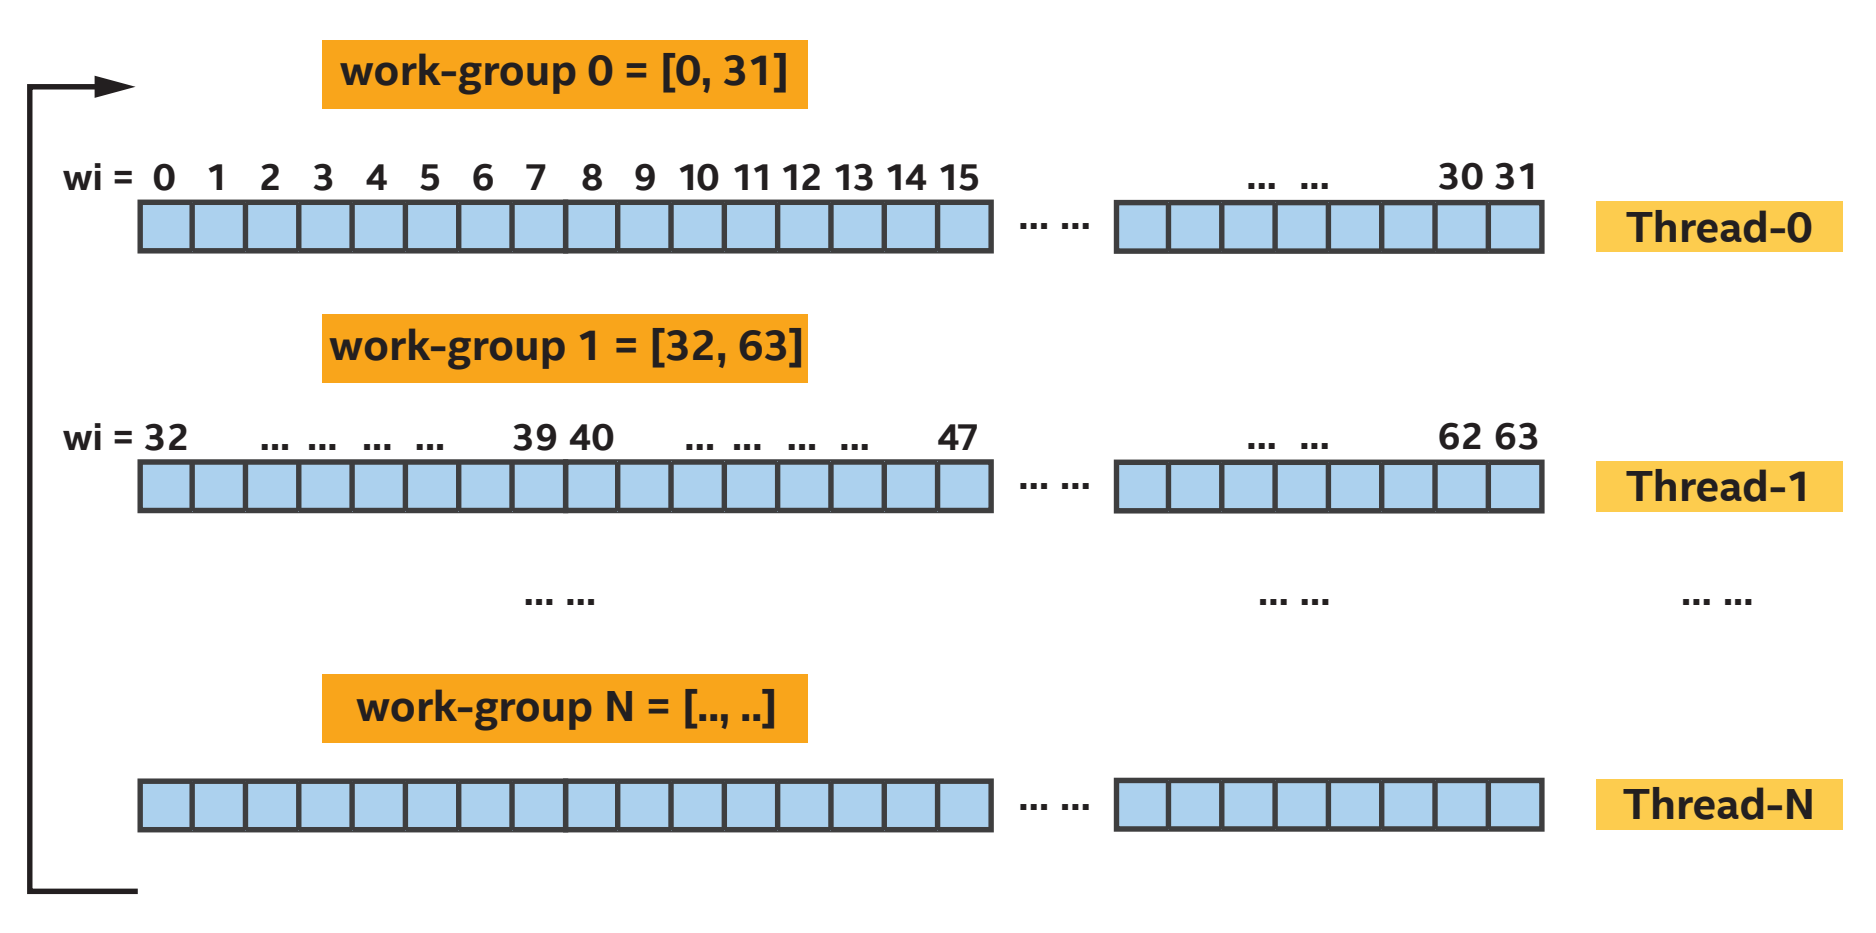
\includegraphics[width=1.0\textwidth]{content/chapter-16/images/5}
\end{center}

Note that in the DPC++ program, the exact way that data elements are partitioned and assigned to different processor cores (or hyper-threads) is not required to be specified. This gives a DPC++ implementation flexibility to choose how best to execute a parallel kernel on a specific CPU. With that said, an implementation can provide some level of control to programmers to enable performance tuning.\par

While a CPU may impose a relatively high thread context switch and synchronization overhead, having somewhat more software threads resident on a processor core is beneficial because it gives each processor core a choice of work to execute. If one software thread is waiting for another thread to produce data, the processor core can switch to a different software thread that is ready to run without leaving the processor core idle.\par

\begin{tcolorbox}[colback=blue!5!white,colframe=blue!75!black, title=CHOOSING HOW TO BIND AND SCHEDULE THREADS]
Choosing an effective scheme to partition and schedule the work among threads is important to tune an application on CPUs and other device types. Subsequent sections will describe some of the techniques.
\end{tcolorbox}

\hspace*{\fill} \par %插入空行
\textbf{Thread Affinity Insight}

Thread affinity designates the CPU cores on which specific threads execute. Performance can suffer if a thread moves around among cores, for instance, if threads do not execute on the same core, cache locality can become an inefficiency if data ping-pongs between different cores.\par

The DPC++ runtime library supports several schemes for binding threads to core(s) through environment variables DPCPP\_CPU\_CU\_AFFINITY, DPCPP\_CPU\_PLACES, DPCPP\_CPU\_NUM\_CUS, and DPCPP\_CPU\_SCHEDULE, which are not defined by SYCL.\par

The first of these is the environment variable DPCPP\_CPU\_CU\_AFFINITY. Tuning using these environment variable controls is simple and low cost and can have large impact for many applications. The description of this 
environment variable is shown in Figure 16-8.\par

\hspace*{\fill} \par %插入空行
Figure 16-8. DPCPP\_CPU\_CU\_AFFINITY environment variable

\begin{table}[H]
	\begin{tabular}{|l|l|}
		\hline
		\textbf{DPCPP\_CPU\_CU\_AFFINITY} & \textbf{Descriiption}                                                                                                                    \\ \hline
		spread                            & \begin{tabular}[c]{@{}l@{}}Bind successive threads to distinct sockets starting with\\ socket 0 in a round-robin order\end{tabular}      \\ \hline
		close                             & \begin{tabular}[c]{@{}l@{}}Bind successive threads to distinct hyper-thread starting\\ with thread 0 in a round-robin order\end{tabular} \\ \hline
	\end{tabular}
\end{table}

\begin{tcolorbox}[colback=green!5!white,colframe=green!75!black]
spread: boundHT = (tid mod numHT) + ( tid mod numSocket) x numHT \\
close: boundHT = tid mod(numSocket x numHT)
\end{tcolorbox}

where\par

\begin{itemize}
	\item tid denotes a software thread identifier.
	\item boundHT denotes a hyper-thread (logical core) that thread tid is bound to.
	\item numHT denotes the number of hyper-threads per socket.
	\item numSocket denotes the number of sockets in the system
\end{itemize}

Assume that we run a program with eight threads on a dual-core dual-socket hyper-threading system—in other words, we have four cores for a total of eight hyper-threads to program. Figure 16-9 shows examples of how threads can map to the hyper-threads and cores for different DPCPP\_CPU\_CU\_AFFINITY settings.\par

\hspace*{\fill} \par %插入空行
Figure 16-9. Mapping threads to cores with hyper-threads
\begin{center}
	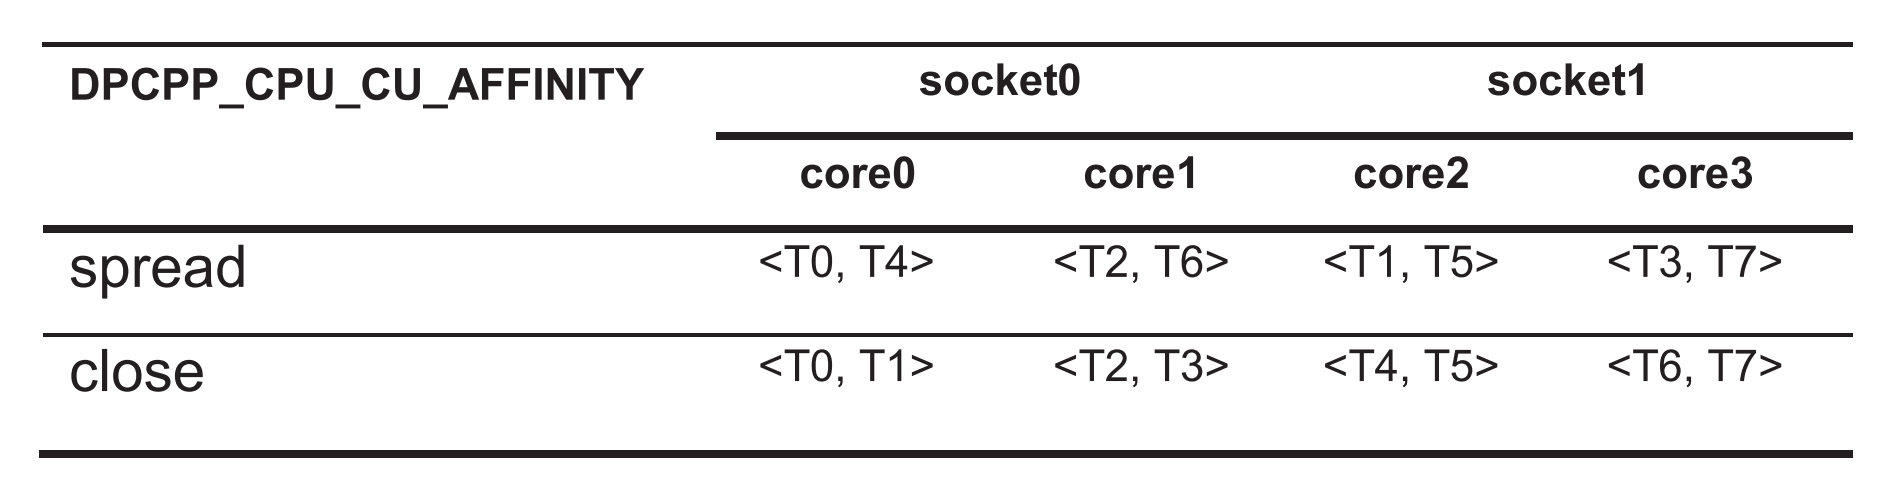
\includegraphics[width=1.0\textwidth]{content/chapter-16/images/6}
\end{center}

In conjunction with the environment variable DPCPP\_CPU\_CU\_AFFINITY, there are other environment variables that support CPU performance tuning:\par

\begin{itemize}
	\item DPCPP\_CPU\_NUM\_CUS = [n], which sets the number of threads used for kernel execution. Its default value is the number of hardware threads in the system.
	\item DPCPP\_CPU\_PLACES = [ sockets | numa\_domains | 	cores | threads ], which specifies the places that the 	affinity will be set similar to OMP\_PLACES in OpenMP 5.1. The default setting is cores.
	\item DPCPP\_CPUSCHEDULE = [ dynamic | affinity | static ], which specifies the algorithm for scheduling work-groups. Its default setting is dynamic.
	\begin{itemize}
		\item dynamic: Enable the TBB auto\_partitioner, which usually performs sufficient splitting to balance the load among worker threads.
		\item affinity: Enable the TBB affinity\_partitioner, which improves cache affinity and uses proportional splitting when mapping subranges to worker threads.
		\item static: Enable the TBB static\_partitioner, which distributes iterations among worker threads as uniformly as possible.
	\end{itemize}
\end{itemize}

The TBB partitioner uses a grain size to control work splitting, with a default grain size of 1 which indicates that all work-groups can be executed independently. More information can be found at spec.oneapi.com/versions/latest/elements/oneTBB/source/algorithms.html\#partitioners.\par

A lack of thread affinity tuning does not necessarily mean lower performance. Performance often depends more on how many total threads are executing in parallel than on how well the thread and data are related and bound. Testing the application using benchmarks is one way to be certain whether the thread affinity has a performance impact or not. The DPC++ STREAM Triad code, as shown in Figure 16-1, started with a lower performance without thread affinity settings. By controlling the affinity setting and using static scheduling of software threads through the environment variables (exports shown in the following for Linux), performance improved:\par

\begin{tcolorbox}[colback=white,colframe=black]
export DPCPP\_CPU\_PLACES=numa\_domains\\
export DPCPP\_CPU\_CU\_AFFINITY=close
\end{tcolorbox}

By using numa\_domains as the places setting for affinity, the TBB task arenas are bound to NUMA nodes or sockets, and the work is uniformly distributed across task arenas. In general, the environment variable DPCPP\_CPU\_PLACES is recommended to be used together with DPCPP\_CPU\_CU\_AFFINITY. These environment variable settings help us to achieve a ~30\% performance gain on a Skylake server system with 2 sockets and 28 two-way hyper-threading cores per socket, running at 2.5 GHz. However, we can still do better to further improve the performance on this CPU.\par

\hspace*{\fill} \par %插入空行
\textbf{Be Mindful of First Touch to Memory}

Memory is stored where it is first touched (used). Since the initialization loop in our example is not parallelized, it is executed by the host thread in serial, resulting in all the memory being associated with the socket that the host thread is running on. Subsequent access by other sockets will then access data from memory attached to the initial socket (used for the initialization), which is clearly undesirable for performance. We can achieve a higher performance on the STREAM Triad kernel by parallelizing the initialization loop to control the first touch effect across sockets, as shown in Figure 16-10.\par

\hspace*{\fill} \par %插入空行
Figure 16-10. STREAM Triad parallel initialization kernel to control first touch effects
\begin{lstlisting}[caption={}]
template <typename T>
void init(queue &deviceQueue, T* VA, T* VB, T* VC, size_t array_size) {
	range<1> numOfItems{array_size};
	
	buffer<T, 1> bufferA(VA, numOfItems);
	buffer<T, 1> bufferB(VB, numOfItems);
	buffer<T, 1> bufferC(VC, numOfItems);
	
	auto queue_event = deviceQueue.submit([&](handler& cgh) {
		auto aA = bufA.template get_access<sycl_write>(cgh);
		auto aB = bufB.template get_access<sycl_write>(cgh);
		auto aC = bufC.template get_access<sycl_write>(cgh);
		
		cgh.parallel_for<class Init<T>>(numOfItems, [=](id<1> wi) {
			aA[wi] = 2.0; aB[wi] = 1.0; aC[wi] = 0.0;
		});
	});

	queue_event.wait();
}
\end{lstlisting}

Exploiting parallelism in the initialization code improves performance of the kernel when run on a CPU. In this instance, we achieve a ~2x performance gain on an Intel Xeon processor system.\par

The recent sections of this chapter have shown that by exploiting thread-level parallelism, we can utilize CPU cores and hyper-threads effectively. However, we need to exploit the SIMD vector-level parallelism in the CPU core hardware as well, to achieve peak performance.\par

\begin{tcolorbox}[colback=blue!5!white,colframe=blue!75!black]
DPC++ parallel kernels benefit from thread-level parallelism across cores and hyper-threads!
\end{tcolorbox}





